%%%%%%%%%%%%%%%%%%%%%%%%%%%%%%%%%%%%%%%%%
% University/School Laboratory Report
% LaTeX Template
% Version 3.1 (25/3/14)
%
% This template has been downloaded from:
% http://www.LaTeXTemplates.com
%
% Original author:
% Linux and Unix Users Group at Virginia Tech Wiki 
% (https://vtluug.org/wiki/Example_LaTeX_chem_lab_report)
%
% License:
% CC BY-NC-SA 3.0 (http://creativecommons.org/licenses/by-nc-sa/3.0/)
%
%%%%%%%%%%%%%%%%%%%%%%%%%%%%%%%%%%%%%%%%%

%----------------------------------------------------------------------------------------
%	PACKAGES AND DOCUMENT CONFIGURATIONS
%----------------------------------------------------------------------------------------

\documentclass{article}
\newcommand{\shellcmd}[1]{\\\indent\indent\texttt{\footnotesize\# #1}\\}
\usepackage{graphicx} % Required for the inclusion of images
\graphicspath{ {images/} }
\usepackage{natbib} % Required to change bibliography style to APA
\usepackage{amsmath} % Required for some math elements 

\setlength\parindent{0pt} % Removes all indentation from paragraphs


%\usepackage{times} % Uncomment to use the Times New Roman font

%----------------------------------------------------------------------------------------
%	DOCUMENT INFORMATION
%----------------------------------------------------------------------------------------

\title{Project 1: Performance Analysis of IPC Paradigms \\ NWEN 401} % Title

\author{Sriram Venkatesh \\ Victoria University of Wellington} % Author name

\date{\today} % Date for the report

\begin{document}

\maketitle % Insert the title, author and date



% If you wish to include an abstract, uncomment the lines below
% \begin{abstract}
% Abstract text
% \end{abstract}

%----------------------------------------------------------------------------------------
%	SECTION 1
%----------------------------------------------------------------------------------------

\section{Introduction}
The goal of the project was to evaluate the performance of the following three inter-process communication mechanisms:

% If you have more than one objective, uncomment the below:
\begin{enumerate}
	\item Java Sockets
	\item Java Remote Method Invocation (Java RMI)
	\item Java Message Service using JBoss Package
\end{enumerate}

For the experiment, I have created a simple Ping application where the client sends an request to the server and the server sends back a response acknowledging the request. \\

\subsection{Problems to be Solved}
After the completion of the experiment, the following questions will be answered:
\begin{itemize}
	\item What is the relative performance of each IPC method?
	\item How does the features of each method explain the difference in performance?	
	\item Does the location (Local Network/Different Network) of the client/server pair affect the performance of the IPC?
\end{itemize}

\subsection{Experiment Scenarios}
Each IPC was tested under the following conditions:
\begin{itemize}
	\item Each client will send 50 requests to the server.
	\item The client and server were run the same local network, and the client and server were run
	on different network.
	\item Tests were all run using a Unix Machine running similar specs. 
	\item For testing under different networks, a SSH Tunnel was created between the remote and local machine.
\end{itemize}

\subsection{Performance Criteria}
For the purposes of this project we have measured the round trip times (RTT) and throughput of each application. The RTT is the total time a method invocation takes. It is important to not that the methods used for perfomrance evaluation do not do any processing and therefore the RTT expresses the overheard of the method invocation. \\

In the each of the test cases, the network is fast and has a high bandwidth. The Client and Server systems under test are running tightly controlled (50) repeated loops of remote method requests. \\

The response time in this distributed configuration is appoximately



 
%----------------------------------------------------------------------------------------
%	SECTION 2
%----------------------------------------------------------------------------------------

\section{Apparatus}

\subsection{Software Used}

\begin{itemize}
\item {\bf Wireshark} was used to derive statistics related to calculate the Round Trip time between the client and server for all the the different IPC paradigms
\end{itemize}


%----------------------------------------------------------------------------------------
%	SECTION 3
%----------------------------------------------------------------------------------------

\section{Procedures}

\subsection{Using Wireshark}
Wireshark was used to derive statistics related to calculate the Round Trip time between the client and server for all the the different IPC paradigms \\

Instructions to use Wireshark Network Protocol Analyzer (Assumes wireshark is already installed):
\begin{enumerate}
	\item Execute the following command: \\
	\shellcmd{sudo wireshark}
	You will need to have super user rights to in order to use wireshark properly.
	
	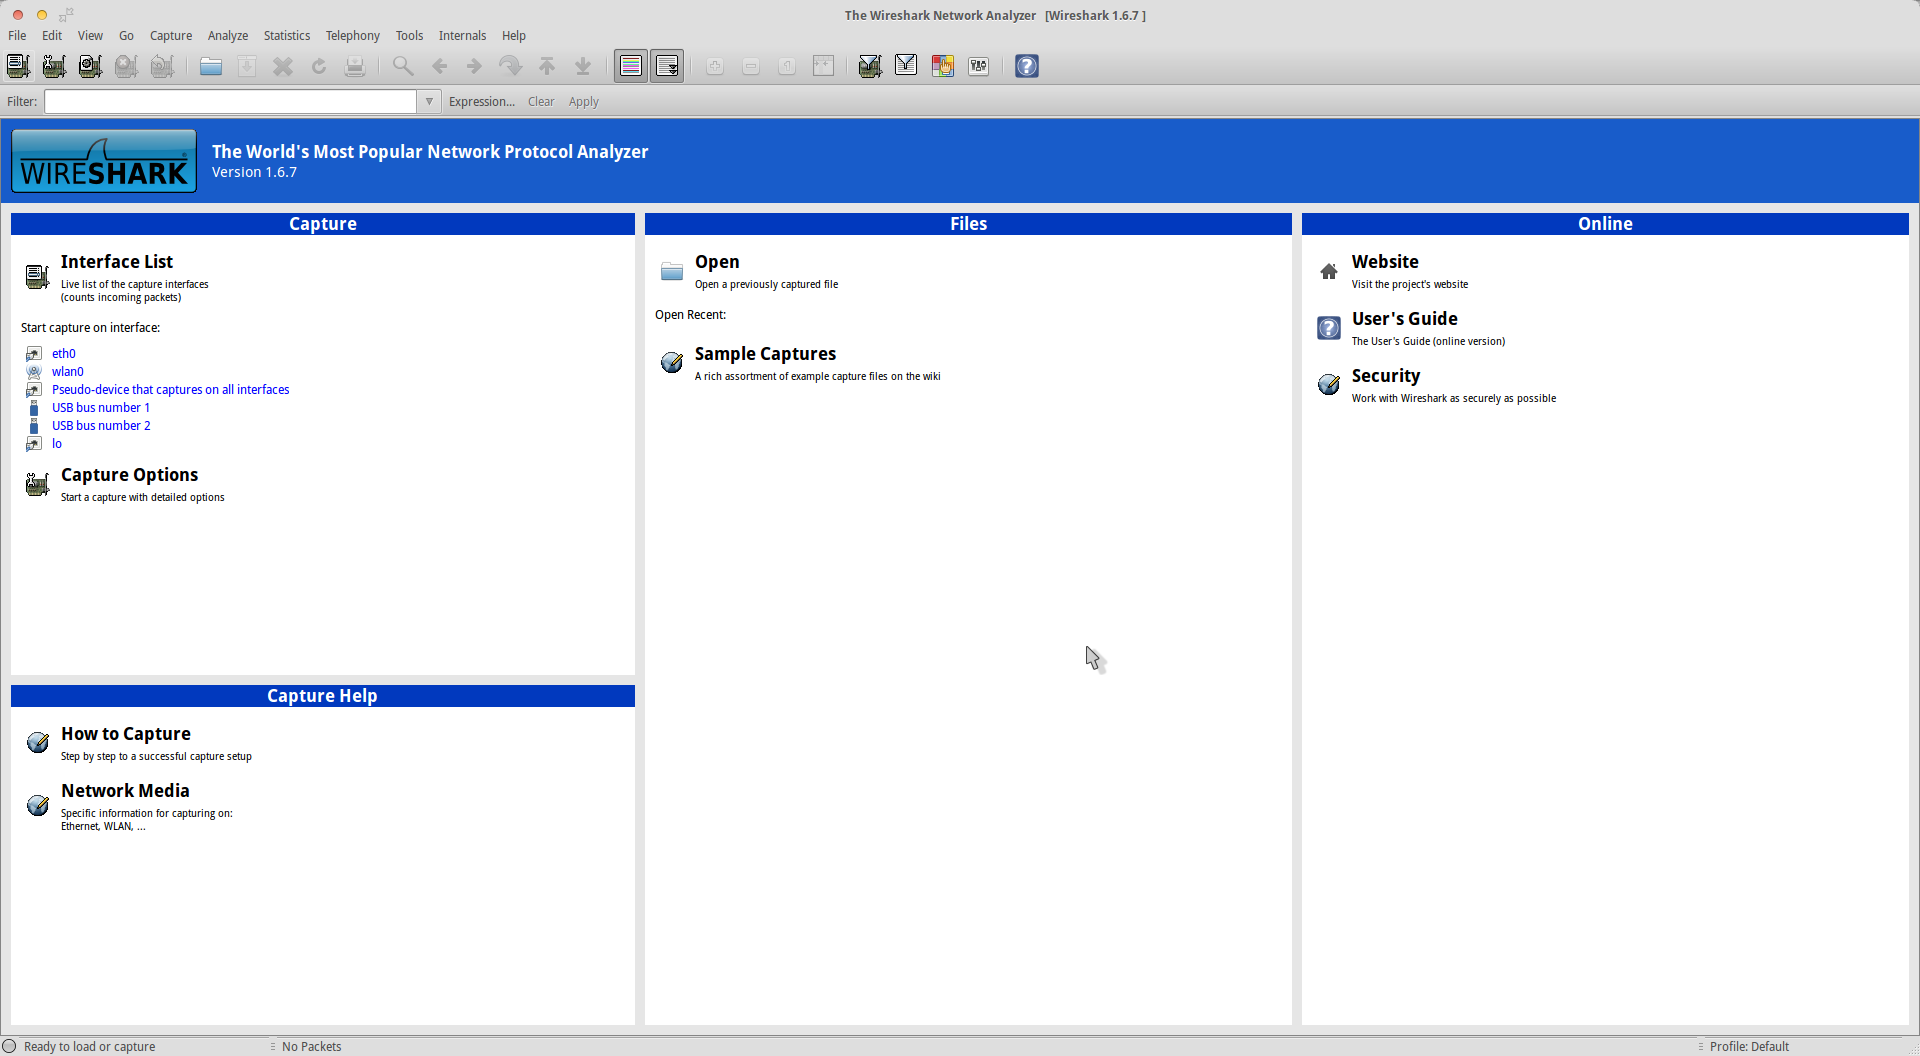
\includegraphics[width=\textwidth]{wireshark-1-screenshot}

	\item Start capturing the traffic on the specfic interface on which you would be running your client application. In this case, it is the wlan0 interface.

	\item After starting capturing on specfic interface, apply filter on it by entering filter expression in filter field at top left corner (as shown below) to capture only traffic between your client and server application.
		\begin{itemize}
        	\item The filter expression for when the client and server are on different networks:
     		\shellcmd{ip.addr==<client-external-ip-address and ip.addr==<host-external-ip-address>}
        	\item The filter expression for when the client and server are on different networks:
     		\shellcmd{ip.addr==<client-internal-ip-address and ip.addr==<host-internal-ip-address>}
    	\end{itemize}

\end{enumerate}


%----------------------------------------------------------------------------------------
%	SECTION 4
%----------------------------------------------------------------------------------------

\section{Performance Results}





%----------------------------------------------------------------------------------------
%	SECTION 5
%----------------------------------------------------------------------------------------

\section{Discussion}


%----------------------------------------------------------------------------------------
%	SECTION 6
%----------------------------------------------------------------------------------------

\section{Conclusions and recommendations}

Performance has an important influence on the usability of distributed applications. Therefore it is useful to know, how well do these distributed models perform. In this project we have clarifed this question. We have compared the relative performance of RMI, JMS and Java Sockets for the Java 7 verion. We have measured the performance on a Linux Computer.

What is the relative performance of each IPC method?


How does the features of each method explain the difference in performance?


Does the location (Local Network/Different Network) of the client/server pair affect the performance of the IPC?



Future projects should compare the relative performance of using these methods of IPC on different operating systems and validate a wheather the operating system affects the performance of these distributed methods.


%----------------------------------------------------------------------------------------
%	BIBLIOGRAPHY
%----------------------------------------------------------------------------------------

\bibliographystyle{apalike}

\bibliography{sample}

%----------------------------------------------------------------------------------------


\end{document}